\documentclass[10pt, compress, aspectratio=169]{beamer}

\usetheme[numbering=fraction, progressbar=none, titleformat=smallcaps]{metropolis}
\usepackage{booktabs}
\usepackage{array}
\usepackage{listings}
\usepackage{graphicx}
\usepackage[scale=2]{ccicons}
\usepackage{url}
\usepackage{relsize}
\usepackage{wasysym}

\usepackage{pgfplots}
\usepgfplotslibrary{dateplot}

\lstset{ %
  backgroundcolor={},
  basicstyle=\ttfamily\footnotesize,
  breakatwhitespace=true,
  breaklines=true,
  captionpos=n,
  commentstyle=\color{orange},
  escapeinside={\%*}{*)},
  extendedchars=true,
  frame=n,
  keywordstyle=\color{orange},
  language=bash,
  rulecolor=\color{black},
  showspaces=false,
  showstringspaces=false,
  showtabs=false,
  numbers=left,
  numbersep=3pt,
  stepnumber=1,
  stringstyle=\color{gray},
  tabsize=2,
  keywords={thrust,plus,device_vector, copy,transform,begin,end, copyin,
  copyout, acc, \_\_global\_\_, void, int, float, main, threadIdx, blockIdx,
  blockDim, if, else, malloc, NULL, cudaMalloc, cudaMemcpy, cudaSuccess,
  cudaGetLastError, cudaDeviceSynchronize, cudaFree, cudaMemcpyDeviceToHost,
  cudaMemcpyHostToDevice, const, data, independent, kernels, loop,
  fprintf, stderr, cudaGetErrorString, EXIT_FAILURE, for, dim3},
  otherkeywords={::, \#pragma, \#include, <<<,>>>, \&, \*, +, -, /, [, ], >, <}
}

\renewcommand*{\UrlFont}{\ttfamily\smaller\relax}

\graphicspath{{images/}}

\title{Using History Interactively}
\author{\footnotesize Rodrigo Siqueira \\ {\scriptsize siqueira@ime.usp.br}}
%\institute{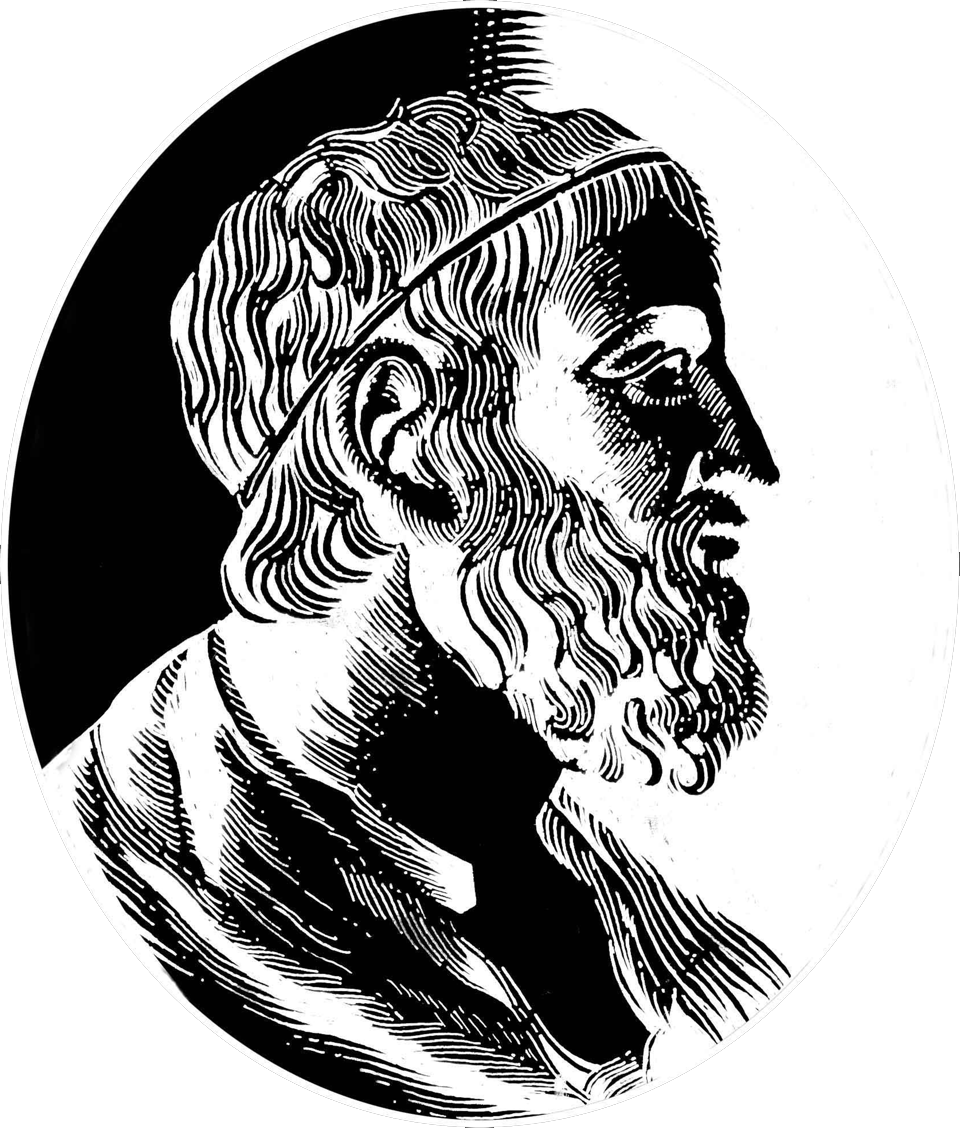
\includegraphics[height=2cm]{imelogo}\\[0.2cm] Department of Computer Science \\ University of São Paulo}

\begin{document}

\maketitle

%------------------------------------------------------------------------------
\section{Section name}
\begin{frame}{Section}
  \metroset{block=fill}
  \begin{exampleblock}{Bases}
    \begin{itemize}
      \item Some stuff here.
      \item Another stuff here..
    \end{itemize}
  \end{exampleblock}
\end{frame}

%------------------------------------------------------------------------------
\section{Another section}

\begin{frame}{Another section}
  \metroset{block=fill}
  \begin{alertblock}{Alert block}
    \begin{itemize}
      \item Some stuff here...
    \end{itemize}
  \end{alertblock}
\end{frame}

%------------------------------------------------------------------------------
\section{About this presentation}
\begin{frame}[standout]
  % TODO: Improve it
   \begin{center}\ccbysa\end{center}
\end{frame}

%TODO: Bibliography
% break [n]: http://tldp.org/LDP/abs/html/loopcontrol.html
% continue [n]: http://tldp.org/LDP/abs/html/loopcontrol.html
% exec: http://wiki.bash-hackers.org/commands/builtin/exec
% caller: http://wiki.bash-hackers.org/commands/builtin/caller
% key num code: http://invisible-island.net/xterm/xterm-function-keys.html
\maketitle

\end{document}
